%\section{Notes and thoughts - to be completed}
For distributed Web3, and by extension metaverse applications to flourish it is necessary to solve the identification problem \cite{king1966fisher}. Without a \href{https://joshgans.medium.com/web3-isnt-going-to-work-without-identification-6aa776d674}{solution to this} bots, scammers, and AI actors will reduce usefulness and usability of and already quite arcane user experience.\par  
This chapter is an oddity because most of traditional DID/SSI isn't really fit for purpose. Distributed self sovereign identity has a great elevator pitch though. Individuals should be empowered through technology to manage their own data, without manipulation or exploitation by centralised corporate behemoths. In practice it's a staggeringly complex proposition which increases risk to the individual, decreases convenience, and despite much work, does not even make much sense in it's own terms. Webs of trust are viable so this means Nostr, \href{https://github.com/project-bitmark/marking/wiki#marking}{Marking}, or Slashtags which will be discussed, but are early products. %Maybe LNURL-Auth can do it. \par 
Thanks to \href{https://github.com/melvincarvalho}{Melvin Carvalho} for advice with this section.
\section{Applications of DID/SSI}
Some of the likely, and discussed applications for DID/SSI are the more inherently private and personally valuable sets of data an individual might generate throughout their life. The theory is that subsets of such data could then be digitally revealed by the individual when required, and that cryptographic verification built into the system would guarantee the veracity of the data to the receiving party. It is also possible to make use of ``zero-knowledge proof'' such that assertions can be made about about the contents of the data without revealing the data itself. A good example of this an age verification challenge, where a threshold age could be asserted without necessarily revealing the date of birth. 
Other keystone uses of the technology are:
\begin{itemize}
\item health documents history
\item qualifications and certifications
\item financial record and relationships with those of others
\item contacts, connections to other people and their appropriate data, including things like shared and personal calendars
\end{itemize}  
It's also possible to extend this key management ethos to all login credentials, and all data currently stored on centralised servers. This is the tension discussed in the chapter about Web3. Proponents think that using something like a DID/SSI stack to manage encryption, decryption and access to data within cloud services gives the user the best of all worlds. They see simply logging in with a cryptographic wallet, and using that same public/private key pair to manage the data beyond as some kind of panacea. This is very complex stuff though, and it seems very likely they just haven't thought this through enough.
\section{Classic DID/SSI}
Distributed identity / self sovereign identity has been extensively researched for decades, with hundreds of peer reviewed papers, and extensive support from the \href{https://www.w3.org/TR/did-core/}{world wide web consortium}. The academic field now seems quite ossified and has settled on a couple of hundred `schema' which they feel underpin the next layer of development. It is a \href{https://medium.com/decentralized-identity/overview-of-decentralized-identity-standards-f82efd9ab6c7}{complex field}, and the language and diagrams are arcane and self referential as seen in Figure \ref{fig:DID}.
\begin{figure}
\includegraphics[width=\linewidth]{DID}
  \caption{Part of the DID SSI specs}
  \label{fig:DID}
\end{figure}. 
Moreover the minimal implementation of such proposed systems hints at a \href{https://www.w3.org/community/perma-id/}{federated model} of \href{https://github.com/w3c/vc-data-model/issues/947#issuecomment-1276186406}{centralised/federated `truth'} to enable persistence of identifiers over time.\\
The major failing of the DID/SSI work to date is a lack of meaningful use cases with incentives for adoption. This is clearly explained by Lockwood \cite{lockwood2021exploring} who proposes that the pathway to adoption of `classic' DID/SSI requires an incentive over and above the current identity management on the web. Being distributed is not enough. Especially in the light of questionable assurances of this even being true.\\
Perhaps most concerning is this \href{https://lists.w3.org/Archives/Public/public-credentials/2022Mar/thread.html}{recent exchange} on the mailing lists. Here, two long standing developers of DID say the following:\\
\textit{``Not a single entity I know that's doing production deployments has actually vetted did:ion and found it to be production capable. This goes for every DLT-based DID Method out there - even the one we're working on. I am highly sceptical of anyone that says that any DID Method is ready for production usage at present.\\
Agreed — as one of the proponents of DLTs (in particular permissionless public ones) none are mature enough yet for production.''}.
It seems then that we can rule out use of these technologies?

\subsubsection{DID principles}
The core principles of distributed identity are that there should be persistent identifiers, like real world documents which assert identity, but with extended use cases. These should be permanent, and resolvable everywhere, forever. Underpinning this is cryptographically verifiable and decentralised data, managed by the user, or their trusted proxy. As primitives this makes them lifetime digital assets, that are portable, and unconfiscatable, with no required reliance on a trusted third party. By this stage in the book you should be familiar with these concepts, but application of this fundamental mindset to all personal data and digital interactions is a bigger reach even than money and value.
\subsubsection{What's in a DID document?}
All classic DID is underpinned by a DID document what bootstrap the services it's connected to. It is made up of one or more public keys. The documents can make use of services such as timestamps, cryptographic signatures, proofs, delegations, and authorisations. They should contain the minimum amount of information to accomplish the specific task required of them.

\section{Newer Technologies}
This section about newer technologies is perhaps best \href{https://www.getrevue.co/profile/jackjack/issues/a-native-internet-protocol-for-social-media-1503112?via=twitter-card&client=DesktopWeb&element=issue-card}{summarised by Jack Dorsey}, ex CEO of twitter, paraphrased here:\\
\textit{``I'll start with the
principles I've come to believe based on everything I've learned and experienced through my past actions as a Twitter co-founder and Lead:
\begin{itemize}
\item Social media must be resilient to corporate and government control.
\item Only the original author may remove content they produce.
\item Moderation is best implemented by algorithmic choice.
\end{itemize} 
The biggest mistake I made was
continuing to invest in building tools
for us to manage the public conversation versus building tools for the people using Twitter to easily manage it for themselves this burdened the company with too much power and opened us to significant outside pressure such as advertising budgets. I generally think companies have become far too powerful. The only way I know of to truly live up to these three principles is a free and open protocol for social media that is not owned by a single company or group of companies and is resilient to corporate and government influence the problem today is that we have companies who own both the protocol and discovery of content which ultimately puts one person in charge of what's available and seen or not this is by definition a single point of failure no matter how great the person and over time will fracture the public conversation and may lead to more control by governments and
corporations around the world.}\par

The following technologies were selected for this book long before Dorsey wrote those words, but they \textit{are} the technologies in which he is investing his time and money to further those 3 principles.
%modelling reputation diagram 2.3.2 %\cite{mui2002computational}
\subsection{Lightning}
It is possible to log into a website using only Lighting, as in \href{https://stacker.news/login?callbackUrl=https://stacker.news/}{Stacker News}.
\subsection{Web5, Bluesky, \& Microsoft ION}
Promisingly Jack Dorsey's company TBD is working on a project \href{https://developer.tbd.website/projects/web5/}{called ``Web5''}. Details are scant but the promise is decentralised and/or self hosted data and identity running on Bitcoin, without recourse to a new token. \textit{``Components include decentralized identifiers (DIDs), decentralized web node (DWNs), self-sovereign identity service (SSIS) and a self-sovereign identity software development kit (ssi-sdk)''}.\par
Web5 leverages the ION identity stack. All this looks to be exactly what our metaverse system requires, but the complexity is likely to be quite high as it is to be built on existing DID/SSI research which is pretty complex and perhaps has problems.\par 
They readily admit they \href{https://atproto.com/guides/identity}{do not have a working solution} at this time: \textit{``At present, none of the DID methods meet our standards fully. Many existing DID networks are permissionless blockchains which achieve the above goals but with relatively poor latency (ION takes roughly 20 minutes for commitment finality). Therefore we have chosen to support did-web and a temporary method we've created called did-placeholder. We expect this situation to evolve as new solutions emerge.''}
\subsubsection{ION} 
While working at Microsoft on ION Daniel Buchner (now working at Square) or Henry Tsai \href{https://github.com/decentralized-identity/ion/blob/master/docs/Q-and-A.md}{said the following}, which is worth quoting verbatim:\par
``While ledger-based consensus systems, on the surface, would seem to provide the same general features as one another, there are a few key differences that make some more suitable for critical applications, like the decentralized identifiers of human beings. Some of these considerations and features are:
\begin{itemize}
\item The system must be open and permissionless, not a cabal of authorities who can exclude and remove participants.
\item The system must be well-tested, and proven secure against attack over a long enough duration to be confident in.
\item The system must produce a singular, independently verifiable record that is as immutable as possible, so that reversing the record the system produces is infeasible.
\item The system must be widely deployed, with nodes that span the globe, to ensure the record is persisted.
\item The system must be self-incentivized, so that nodes continue to operate, process, and secure the record over time. The value from operation must come from the system directly, because outside incentive reliance is itself a vector for attack.
\item The cost to attack the system through any game theoretically available means must be high enough that it is infeasible to attempt, and even if an ultra-capitalized attacker did, it would require a weaponized mobilization of force and resources that would be obvious, with options for mitigation.\par

The outcome:

\item Number 1 eliminates private and permissioned ledgers
\item Number 2 eliminates just about all other ledgers and blockchains, simply because they are inadequately tested
\item For the metrics detailed in 3-6, Bitcoin is so far beyond all other options, it isn't even close - Bitcoin is the most secure option by an absurdly large margin.''
\end{itemize}

On the surface then it might seem that the choice is Bitcoin again, and indeed that the open source Microsoft ION stack is a natural choice, but it's complex to run, the interactions with the blockchain have a cost implication which can't be surmounted without every user owning some Bitcoin, and as we have seen, there is no formal validation of this system. In addition (in the current implementation) an identity proof does not need to be published to be valid, just timestamped. In this way an identity can be stolen and used years later to claim later chains of proof. It seems that it might be somewhat useful `at scale' and is worth additional monitoring and investigation, especially given it's integration into TBD - Web5.
\subsection{Nostr}
Nostr is ``The simplest open protocol that is able to create a censorship-resistant global "social" network once and for all.'' according to it's \href{https://github.com/fiatjaf/nostr}{github page}. More than that it's a client side validated proof of who a user is interacting with, hence being in this identity section. To be clear, it's not a completely peer to peer system in that it uses relay servers, but this gives it some of the best characteristics of both paradigms. This has the following advantages for our metaverse application; 
\begin{itemize}
\item it's lightweight, with minimal network overhead and complexity
\item it's real-time using websockets
\item anyone can run a relay server, so one can be run in the deployment in the final section of the book.
\item Each of the client peers connecting to the metaverse can be a relay and able to pass messages and proofs to the other clients without the metaverse server seeing the data or being online 
\item it's opensource
\item there are multiple usable libraries and tools
\item it's under active development with an excellent team. The lead, `Fiatjaf' is one of the most \href{https://github.com/fiatjaf}{prolific developers} in the lightning space.
\item it's based on the same underlying cryptographic technology we are using elsewhere, indeed with it's use of Bitcoin keys the identity system is global
\item it provides the identity proof that we need to validate users and objects into a virtual space
\item it enables message passing
\item it scales to be a social network as required
\item it need not rely on anything outside of a relay hosted on the metaverse server
\item it can likely be scaled to provide one to many bulletin board style applications within the metaverse
\item it can easily operate outside of the walled garden of the metaverse, extending the reach of the messages
\end{itemize} 
\href{https://www.forbes.com/sites/rogerhuang/2022/12/29/nostr-is-the-decentralized-protocol-that-might-replace-elon-musks-twitter/?sh=79e2b2be442a}{Nostr is incredibly promising}, and integrating these relays in the metaverse servers and clients of the proposed technology stack in this book might allow us globally provable identity, with privacy by design. It can provide message passing. If all entities in the metaverse scenegraphs are also Nostr key pairs then schema can be applied consistently with the economic layer using the same key system as Bitcoin. Nostr has just received a substantial grant from Dorsey. It is core to the design later in the book. A curated list of projects and libraries is \href{https://github.com/aljazceru/awesome-nostr}{available on github}.\par
\subsection{Slashtags}
Slashtags is a new distributed identity open method being developed by Bitfinex and Tether under the Synonym suite. It uses Bitcoin keys for authentication, but communicates a schema through a metadata exchange.\\
This section needs a rebuild as they have landed a terrific ecosystems and we will certainly have to integrate some of it.
%Can we pair this with \href{https://cblgh.org/trustnet/}{trustnet}?
\subsubsection{Anigma}
Anigma is a Nostr based clone of popular messenger client Telegram. This provides a web2 interface into the metaverse providing:
\begin{itemize}
\item simple cryptographic identity assurance
\item private peer to peer chat
\item group chats and channels
\item email to private message relay
\item links into media on web2 hosts
\end{itemize}
The proposed integration of Nostr, LnBit, Vircadia, and Bitcoin is the core value proposition of this book, with Anigma the final component.
\section{Federated social media trust}
Keybase provides a model of \href{https://book.keybase.io/account#proofs}{importing proofs} from various social media sites. This allows importing of reputation into new ecosystems.
\section{Micropayment based web}
It seems the war against disinformation is now being lost. Much is written in the media about Deepfake technology creating plausible fake videos, but probably more pernicious is the use of toolkits to create entire plausible fake news sites using natural language AI such as GPT3. This makes it cheap to publish potentially market moving news which is then rehypothecated by online news vendors who are hungry for clicks. As these pipelines become more mature it will be difficult to keep fake news for financial or political gain out of the system. One interesting way to do this that \textit{isn't} webs of trust or true cryptographic identity is to charge micropayments for ``one to many'' publication models. This would imply a tiny instant payment for clicks, especially on social media sites such as twitter. This kind of model has been discussed but is only possible in the context of systems such as Lightning where instant micropayment can be realised. It seems possible that this would price out speculative `noise' spam from the information space. It's interesting and ironic that the origin of proof of work was to underpin just such a spam defeating system  \cite{dwork1992pricing}, and that Nakamoto \href{https://www.metzdowd.com/pipermail/cryptography/2009-January/015014.html}{mentioned this application for Bitcoin} back in 2009. There is now much chatter about the integration of Bitcoin with Twitter in light of Musks buyout of the social network.
%\subsection{Open World assumption}
%\href{https://en.wikipedia.org/wiki/Open-world_assumption}{this needs unpacking}
%------------------------------------------------
%\section{File storage}
%This is a tricky section as nothing seems to work. Come back later.
%https://fiatjaf.com/d5031e5b.html
\begin{figure}
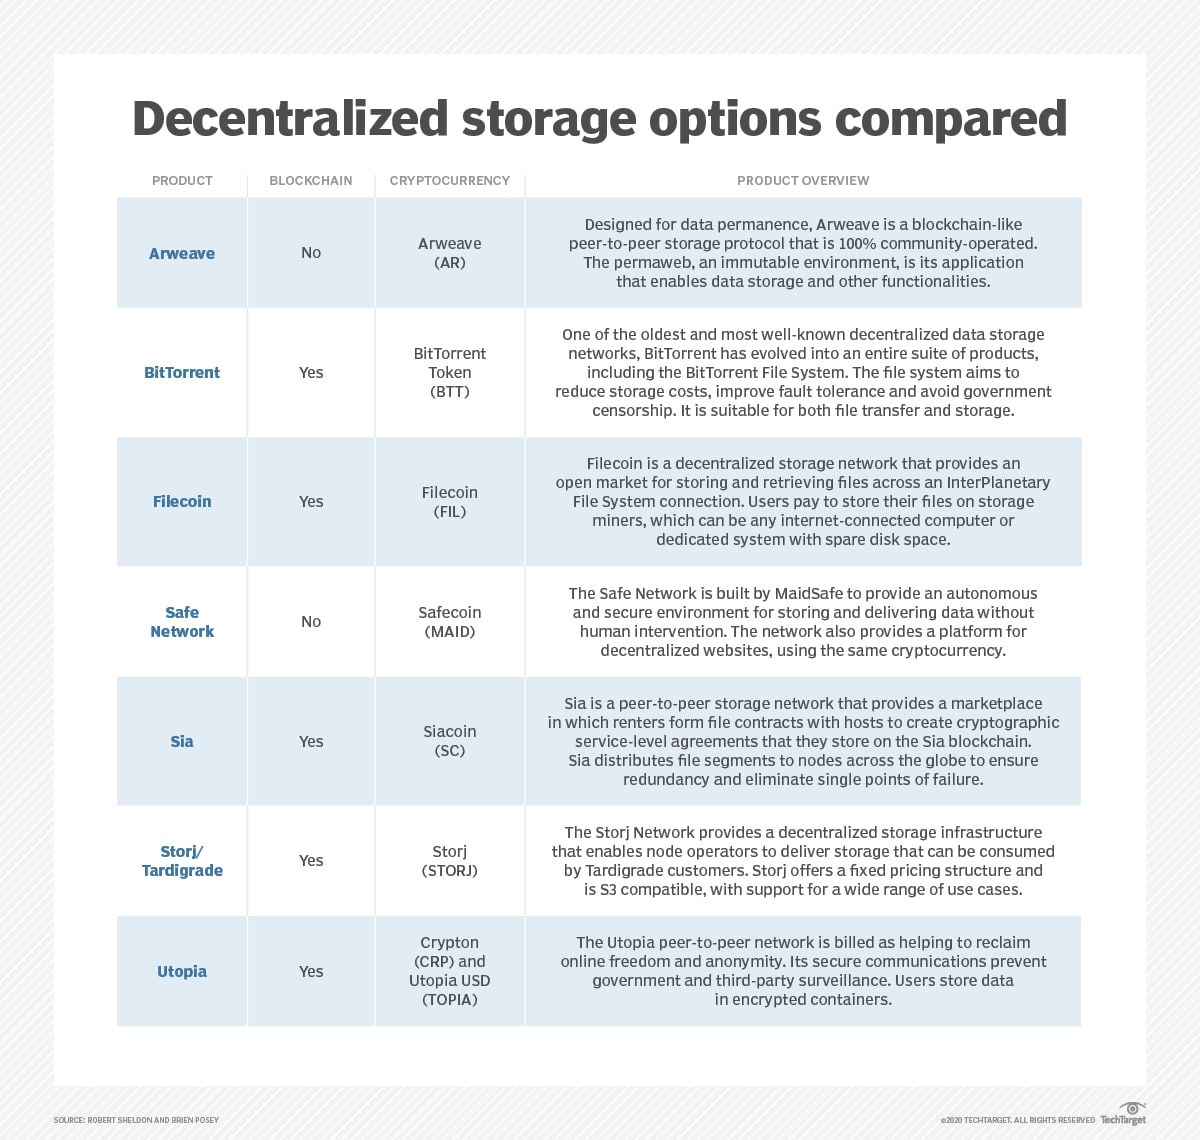
\includegraphics[width=\linewidth]{files}
  \caption{Comparison of distributed file stores}
  \label{fig:Files}
\end{figure}. 
\section{Are DAOs useful for us?}
A distributed autonomous organisation, or DAO is a governance structure which is built in distributed code on a blockchain smart contract system. Token holders have voting rights proportional to their holding. The first decentalised autonomous organisation was simply called ``The DAO'' and was launched on the Ethereum network in 2016 after raising around \$100M. \href{https://www.gemini.com/cryptopedia/the-dao-hack-makerdao#section-what-is-a-dao}{It quickly succumbed to a hack and the money was drained}. This event was an important moment in the development of Ethereum and resulted in a code fork which preserves two separate versions of the network to this day, though one is falling into obsolescence. Again, this is covered in Shin's book on the period in extreme detail, but it seems this stuff is falling into dusty history now, leaving only a somewhat tarnished and technically shaky legacy \cite{cryptopians}. \\
In practice DAOs have very few committed `stakeholders' and the same names seem to crop up across multiple projects. Some crucial community decisions within large projects only poll a couple of dozen eligible participants. Its might be that the experiment of distributed governance is failing at this stage. \par
Perhaps more interesting is the use of the DAO concept to crowd fund global projects, currently especially for the acquisition of important art or cultural items. DAOs are also emerging as a way to fund promising technology projects, though this is reminiscent of the 2017 ICO craze which ended badly and is likely to \href{https://www.cftc.gov/PressRoom/PressReleases/8590-22}{fall foul of regulations}.\par
Within the NFT and digital art space  PleaserDAO has quickly established a strong following.
``PleasrDAO is a collective of DeFi leaders, early NFT collectors and digital artists who have built a formidable yet benevolent reputation for acquiring culturally significant pieces with a charitable twist.\par
Opensea wrangle between IPO and governance token.\par
ConstitutionDAO, Once upon a time in Shaolin etc 
%https://harpers.org/archive/2015/01/come-with-us-if-you-want-to-live/

\subsection{Bisq DAO}
One of the better designed DAOs is \href{https://bisq.network/dao/}{Bisq DAO}. It's slightly different design trys to address the issue of overly rigid software intersecting with more intangible and fluid human governance needs. From their website:\par
\textit{``Revenue distribution and decision-making cannot be decentralized with traditional organization structures—they require legal entities, jurisdictions, bank accounts, and more—all of which are central points of failure.
The Bisq DAO replaces such legacy infrastructure with cryptographic infrastructure to handle project decision-making and revenue distribution without such central points of failure.''}

\subsection{Risks}

The most interesting thing about DAOs is that they belong more in this money chapter than they do in blockchain. As we have seen they're finding most success as loosely regulated crowd funding platforms. If a small company did find itself wishing to explore this fringe mechanism for raising capital, then we would certainly recommend keeping a global eye on evolving regulation and the onward legal exposure of the company. 
\section{Risks \& Challenges?}
Classic DID/SSI risks fragmentations. 
In all DID applications, scaling to a world where the user is managing potentially thousands of these critical cryptographic data files is daunting.
Abstracting the guts of this away to make the use simple, and only mindful of thet right level of information, turns out to be huge problem that nobody has solved
It's not clear that users want this. 
In the case of web of trust like Slashtags it's a big piece of work for the users to rate all of their digital interactions with a trust metric.


